%-----------------------------------------------------------------------------%
% Document class
%-----------------------------------------------------------------------------%
\documentclass[a4paper,12pt,onecolumn,final]{article}
%-----------------------------------------------------------------------------%
% Geometry package for setting page margins
%-----------------------------------------------------------------------------%
\usepackage[paper=a4paper,vscale=0.8,hscale=0.85,centering]{geometry}
%-----------------------------------------------------------------------------%
% Helvet package for font
%-----------------------------------------------------------------------------%
\usepackage[scaled=0.92]{helvet}
\renewcommand{\familydefault}{\sfdefault}
%-----------------------------------------------------------------------------%
% Include special packages here
%-----------------------------------------------------------------------------%
\usepackage{amsmath,amsfonts,amssymb}
\usepackage{xcolor}
\usepackage{graphicx}
\usepackage{hyperref}
\usepackage{listings}
\lstset {backgroundcolor=\color{black!5}, basicstyle=\footnotesize, stringstyle=\color{red}, commentstyle=\color{green!50!black}, basicstyle=\footnotesize\ttfamily, keywordstyle=\color{blue}, 
}
%-----------------------------------------------------------------------------%


%-----------------------------------------------------------------------------%
\begin{document}
%-----------------------------------------------------------------------------%


%-----------------------------------------------------------------------------%
\noindent
\begin{tabular}{|p{0.2\textwidth}|p{0.75\textwidth}|}
\hline
\textbf{G14CAM} & \textbf{Computational Applied Mathematics}
\\
2017--2018 & \textcolor{red}{Coursework 1 Part A}
\\
\hline
\textbf{Name} & \textcolor{red}{Ella Taylor}
\\ 
\textbf{Student ID} & \textcolor{red}{4290562}
\\ 
\textbf{Date} & \today
\\
\hline
\textbf{Existing codes} & \textcolor{red}{Names of approved existing codes that you used}
\\
\hline
\end{tabular}
%-----------------------------------------------------------------------------%
~\\
~\\
\textcolor{red}{LaTeX instruction: This TeX-file template can be compiled using PDFLaTeX.}
\\
%-----------------------------------------------------------------------------%
\section*{Problem 1}
\subsection*{Problem 1.A}
Your solution to problem 1.A could be typed in LaTeX. You can use LaTeX commands for typing symbols (e.g.: $M \alpha \tau \hbar$) and equations:
%
\begin{equation}
    y = y_h + \mathcal{O}(h^p) 
\end{equation}
%
See the \href{https://www.ctan.org/tex-archive/info/lshort/english/?lang=en}{\underline{LaTeX manual (https://www.ctan.org/tex-archive/info/lshort/english/?lang=en)}} for more help.
\par
Alternatively, you can include scans of hand written material:
\\
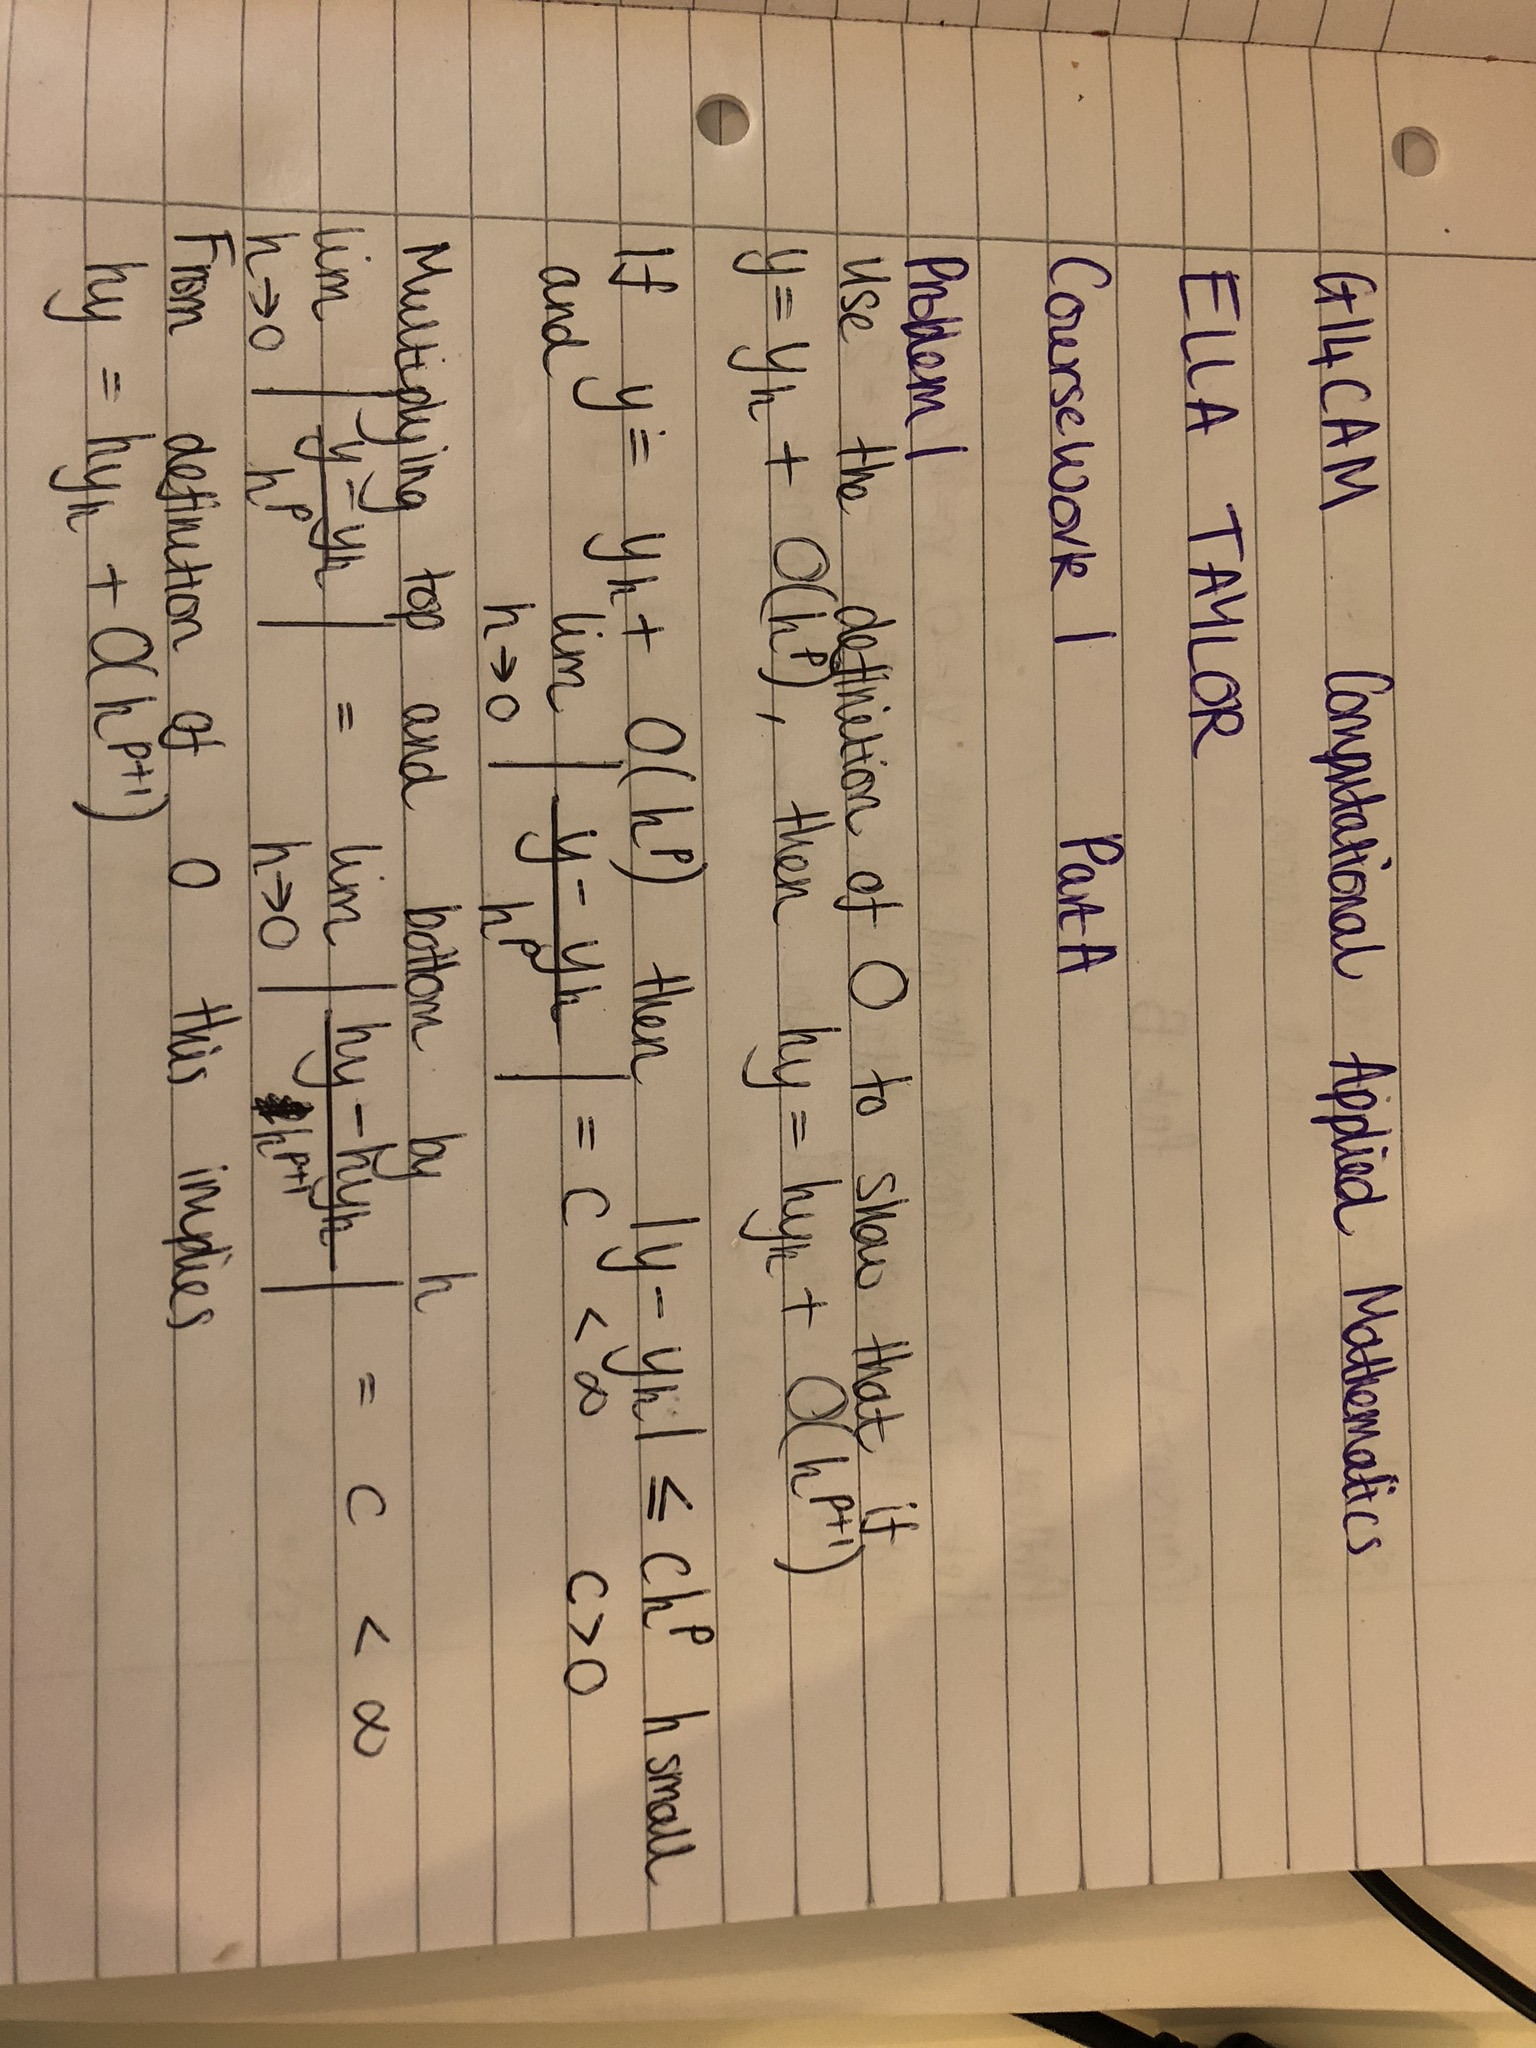
\includegraphics[width=1\textwidth]{../Desktop/01d0f17d133b78915f6aaf5e5dc1ea96222dbe899c.jpg}
%-----------------------------------------------------------------------------%
\section*{Problem 2}
\subsection*{Problem 2.A}

\begin{lstlisting}[language=C++]
#include <iostream>

//Writing a code that implements the tridiagonal matrix algorithm for 
solving an nxn matrix

void tridiagonal_matrix_solver(int n, double* x, double* lower, double* diag, 
double* upper, double* f)
    {
    //Elimination stage

    //f[0] = f[0] and d[0] = d[0] no change
    for (int i = 1; i<n; i++)
        {
        diag[i] = diag[i] - ((upper[i-1]*lower[i-1])/diag[i-1]);
        f[i]    = f[i] - ((f[i-1]*lower[i-1])/diag[i-1]);
        }

    //Backsolving
    //Bottom row is a special case
    x[n-1] = f[n-1]/diag[n-1];

    for (int i = n-2; i >= 0; i--)
        {
        x[i] = (f[i] - upper[i]*x[i+1])/diag[i];
        }

    }

\end{lstlisting}%

%-----------------------------------------------------------------------------%
\subsection*{Problem 2.B}
\begin{center}

\begin{lstlisting}[language=C++]

#include <iostream>
#include <ctime>

void tridiagonal_matrix_solver(int n, double*x, double* lower, double* diag, 
double* upper, double* f);

int main()
{
int n;
std::cout<< "Enter an integer n \n";
std::cin>>n;

double* lower;
lower = new double[n-1];

double* diag;
diag = new double[n];

double* upper;
upper = new double[n-1];

double* f;
f = new double[n];

double* x;
x = new double[n];

x[0] = 0;
diag[0] = 4;
upper[0] = 2;
f[0] = 1;
lower[n-2] = 2;
diag[n-1] = 4;
f[n-1] = (double)(n);
x[n-1] = 0;

for (int i=1; i<n-1; i++)
    {
    x[i] = 0;
    lower[i-1] = 1;
    diag[i] = 4;
    upper[i] = 1;
    f[i] = (double)(i)+1;
    }

clock_t start_s = clock();
tridiagonal_matrix_solver(n,x,lower,diag,upper,f);
clock_t stop_s = clock();
std::cout<<"Time = "<<(stop_s - start_s)/((double)(CLOCKS_PER_SEC))<<"\n";

std::cout<<"x[1] = "<<x[0]<<"\n";
std::cout<<"x[n] = "<<x[n-1]<<"\n";

delete[] lower;
delete[] upper;
delete[] diag;
delete[] f;
delete[] x;

return 0;
}

\end{lstlisting}%


\begin{center}
\begin{tabular}{|c|ccccccc|}
\hline\hline
 $n$ &  2 & 3 & 4 & 8 & 16 & 1,000 & 1,000,000
\\
\hline
 $x_1$ & 0 & 0.0833333 & 0.0666667 & 0.0704225 & 0.0704416 & 0.0704416 & 0.0704416
\\ 
 $x_n$ & 0.5 & 0.583333 & 0.766667 & 1.42958 & 2.76289 & 166.763 & 166,667
\\
\hline\hline
\end{tabular}
\end{center}
%-----------------------------------------------------------------------------%
\subsection*{Problem 2.C}

\begin{tabular}{|c|cccccc|}
\hline\hline
 $n$ &  10^6 & 2x10^6 & 5x10^6 & 10^7 & 1.5x10^7 & 2x10^7
\\
\hline
 $Time$ & 3.8x10^-2 & 7.9x1-^-2 & 1.95x10^-1 & 3.87x10^-1 & 5.71x10^-1 & 7.6x10^-1 
\\
\hline\hline
\end{tabular}
\end{center}

\begin{verbatim}
Plotting a graph of these results it is clear that the relationship between n and 
computational effort is linear (alpha = 1)
\end{verbatim}

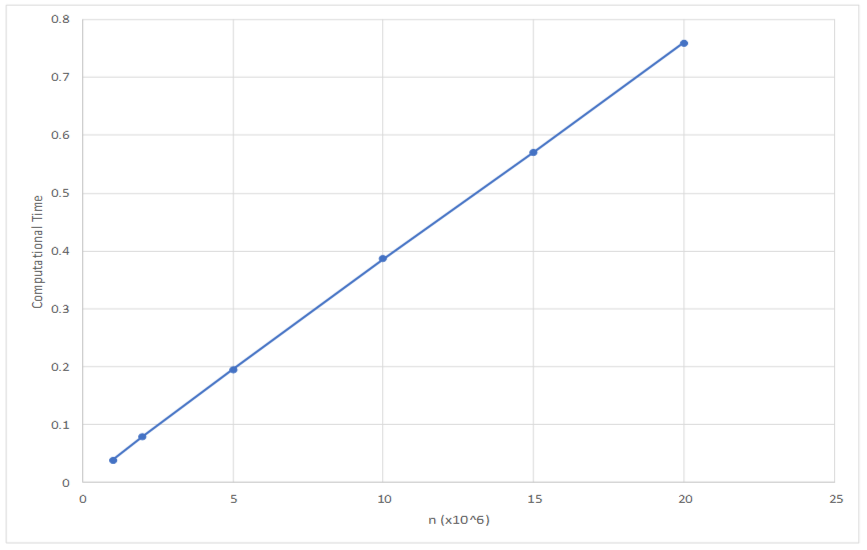
\includegraphics[scale=1]{../Desktop/CAM/CAM_CW1A_Q2C.png} 

\begin{verbatim}
On Wikipedia it says that the standard Gaussian Elimination Algorithm has arithmetic 
complexity O(n^3) so has significantly more computations than the tridiagonal matrix 
algorithm as n increases
\end{verbatim}
%-----------------------------------------------------------------------------%
\end{document}
%-----------------------------------------------------------------------------%
